% pipeline_phase1.tex — the implemented model (Phase 1).
% Standalone TikZ; compile with:  pdflatex pipeline_phase1.tex
\documentclass[tikz,border=6pt]{standalone}
\usepackage{amsmath,amssymb}
\usetikzlibrary{positioning,arrows.meta,fit,backgrounds}

\definecolor{ink}{HTML}{1A1A1A}
\definecolor{muted}{HTML}{6B7280}
\definecolor{rule}{HTML}{9CA3AF}
\definecolor{accent}{HTML}{9A3324}

\begin{document}
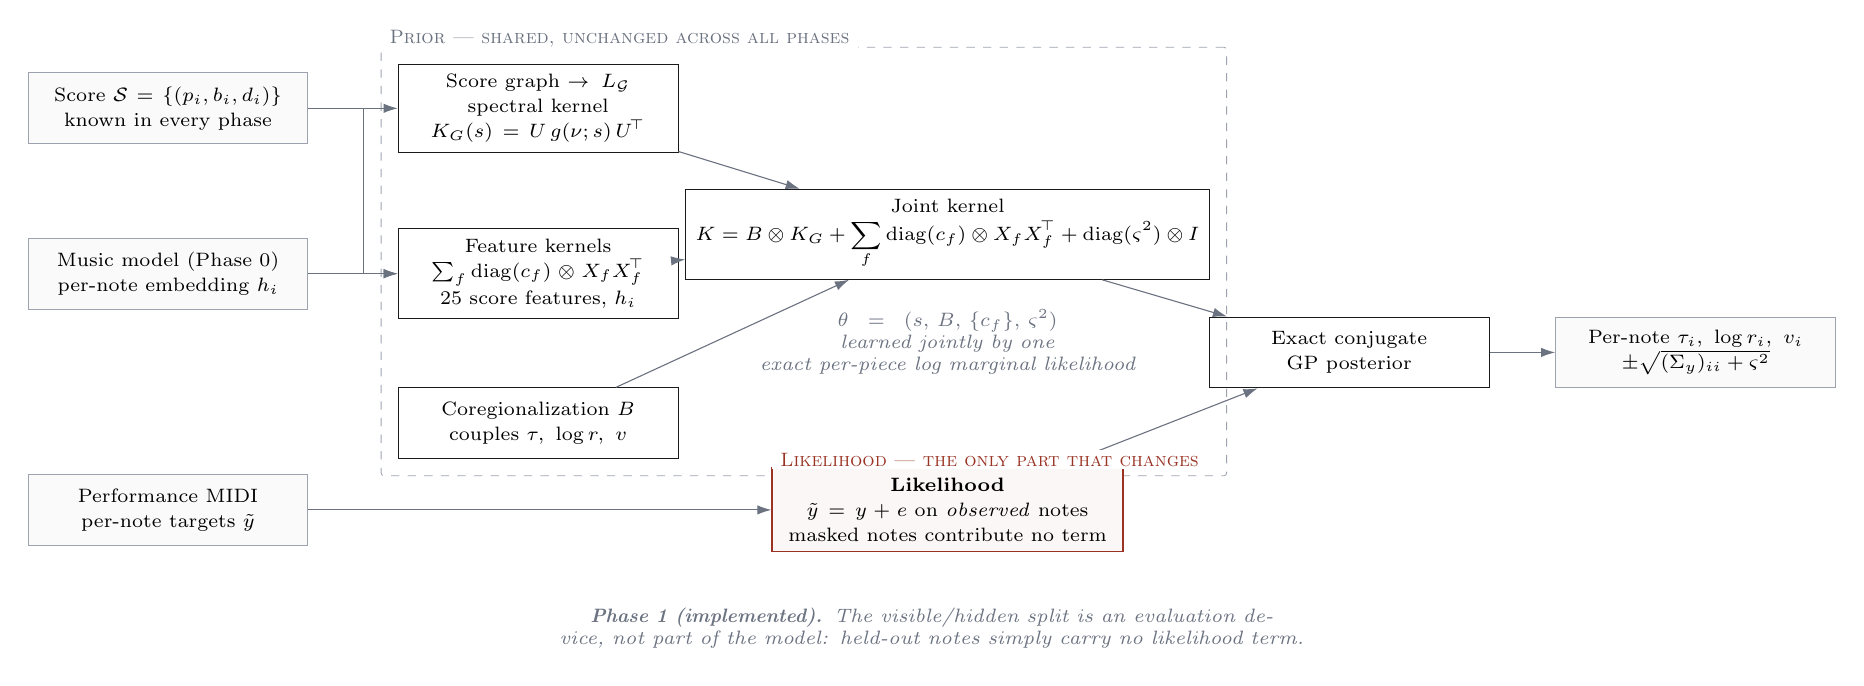
\begin{tikzpicture}[
  font=\scriptsize,
  box/.style   = {draw=ink, line width=0.35pt, align=center, inner sep=3.6pt,
                  text width=33mm, minimum height=9mm},
  io/.style    = {box, draw=rule, fill=black!2},
  acc/.style   = {box, draw=accent, line width=0.6pt, fill=accent!4},
  arr/.style   = {-{Latex[length=1.8mm,width=1.2mm]}, draw=muted, line width=0.4pt},
  note/.style  = {font=\scriptsize\itshape, text=muted, align=center},
  grouplab/.style = {font=\scriptsize\scshape, text=muted, fill=white, inner xsep=3pt, inner ysep=1pt},
]

% ---------- inputs ----------
\node[io] (score) at (0,2.5)
  {Score $\mathcal{S}=\{(p_i,b_i,d_i)\}$\\[1pt] known in every phase};
\node[io] (mm) at (0,0.4)
  {Music model (Phase 0)\\[1pt] per-note embedding $h_i$};
\node[io] (obs) at (0,-2.6)
  {Performance MIDI\\[1pt] per-note targets $\tilde y$};

% ---------- prior construction ----------
\node[box] (gk) at (4.7,2.5)
  {Score graph $\to L_{\mathcal G}$\\[1pt] spectral kernel\\[1pt] $K_G(s)=U\,g(\nu;s)\,U^{\!\top}$};
\node[box] (fk) at (4.7,0.4)
  {Feature kernels\\[1pt] $\textstyle\sum_f \operatorname{diag}(c_f)\otimes X_fX_f^{\!\top}$\\[1pt] 25 score features, $h_i$};
\node[box] (cor) at (4.7,-1.5)
  {Coregionalization $B$\\[1pt] couples $\tau,\ \log r,\ v$};

\node[box, text width=64mm] (K) at (9.9,0.9)
  {Joint kernel\\[2pt]
   $K=B\otimes K_G+\displaystyle\sum_f \operatorname{diag}(c_f)\otimes X_fX_f^{\!\top}+\operatorname{diag}(\varsigma^2)\otimes I$};

% ---------- likelihood (the part that changes) ----------
\node[acc, text width=42mm] (lik) at (9.9,-2.6)
  {\textbf{Likelihood}\\[1pt] $\tilde y = y + e$ on \emph{observed} notes\\[1pt]
   masked notes contribute no term};

% ---------- inference + outputs ----------
\node[box] (inf) at (15.0,-0.6)
  {Exact conjugate\\[1pt] GP posterior};
\node[io] (out) at (19.4,-0.6)
  {Per-note $\tau_i,\ \log r_i,\ v_i$\\[1pt] $\pm\sqrt{(\Sigma_y)_{ii}+\varsigma^2}$};

% ---------- arrows ----------
\draw[arr] (score) -- (gk);
\draw[arr] (score.east) -- ++(0.7,0) |- (fk.west);
\draw[arr] (mm) -- (fk);
\draw[arr] (gk) -- (K);
\draw[arr] (fk) -- (K);
\draw[arr] (cor) -- (K);
\draw[arr] (obs) -- (lik);
\draw[arr] (K) -- (inf);
\draw[arr] (lik) -- (inf);
\draw[arr] (inf) -- (out);

% ---------- annotations ----------
\node[note, below=2.5mm of K, text width=52mm]
  {$\theta=(s,\,B,\,\{c_f\},\,\varsigma^2)$ learned jointly by one\\ exact per-piece log marginal likelihood};

\begin{scope}[on background layer]
  \node[draw=rule, dashed, line width=0.3pt, rounded corners=1pt,
        fit=(gk)(fk)(cor)(K), inner sep=6pt] (prior) {};
\end{scope}
\node[grouplab, above=1mm of prior.north west, anchor=west]
  {Prior --- shared, unchanged across all phases};
\node[grouplab, text=accent, above=1mm of lik.north west, anchor=west]
  {Likelihood --- the only part that changes};

\node[note, text width=150mm] at (9.7,-4.1)
  {\textbf{Phase 1 (implemented).} The visible/hidden split is an evaluation device, not part of the model:
   held-out notes simply carry no likelihood term.};

\end{tikzpicture}
\end{document}
